



\begin{figure}[H] %h:Grafik an dieser Stelle einbinden. Falls das nicht geht: %t:oben auf der Seite. Wenn dies auch nicht möglich ist: %b:am Fuß der Seite oder %p:auf der nächsten Seite %! is specified, then ignore the restrictions of placing floating objects %H (float package) forces position
  \centering
     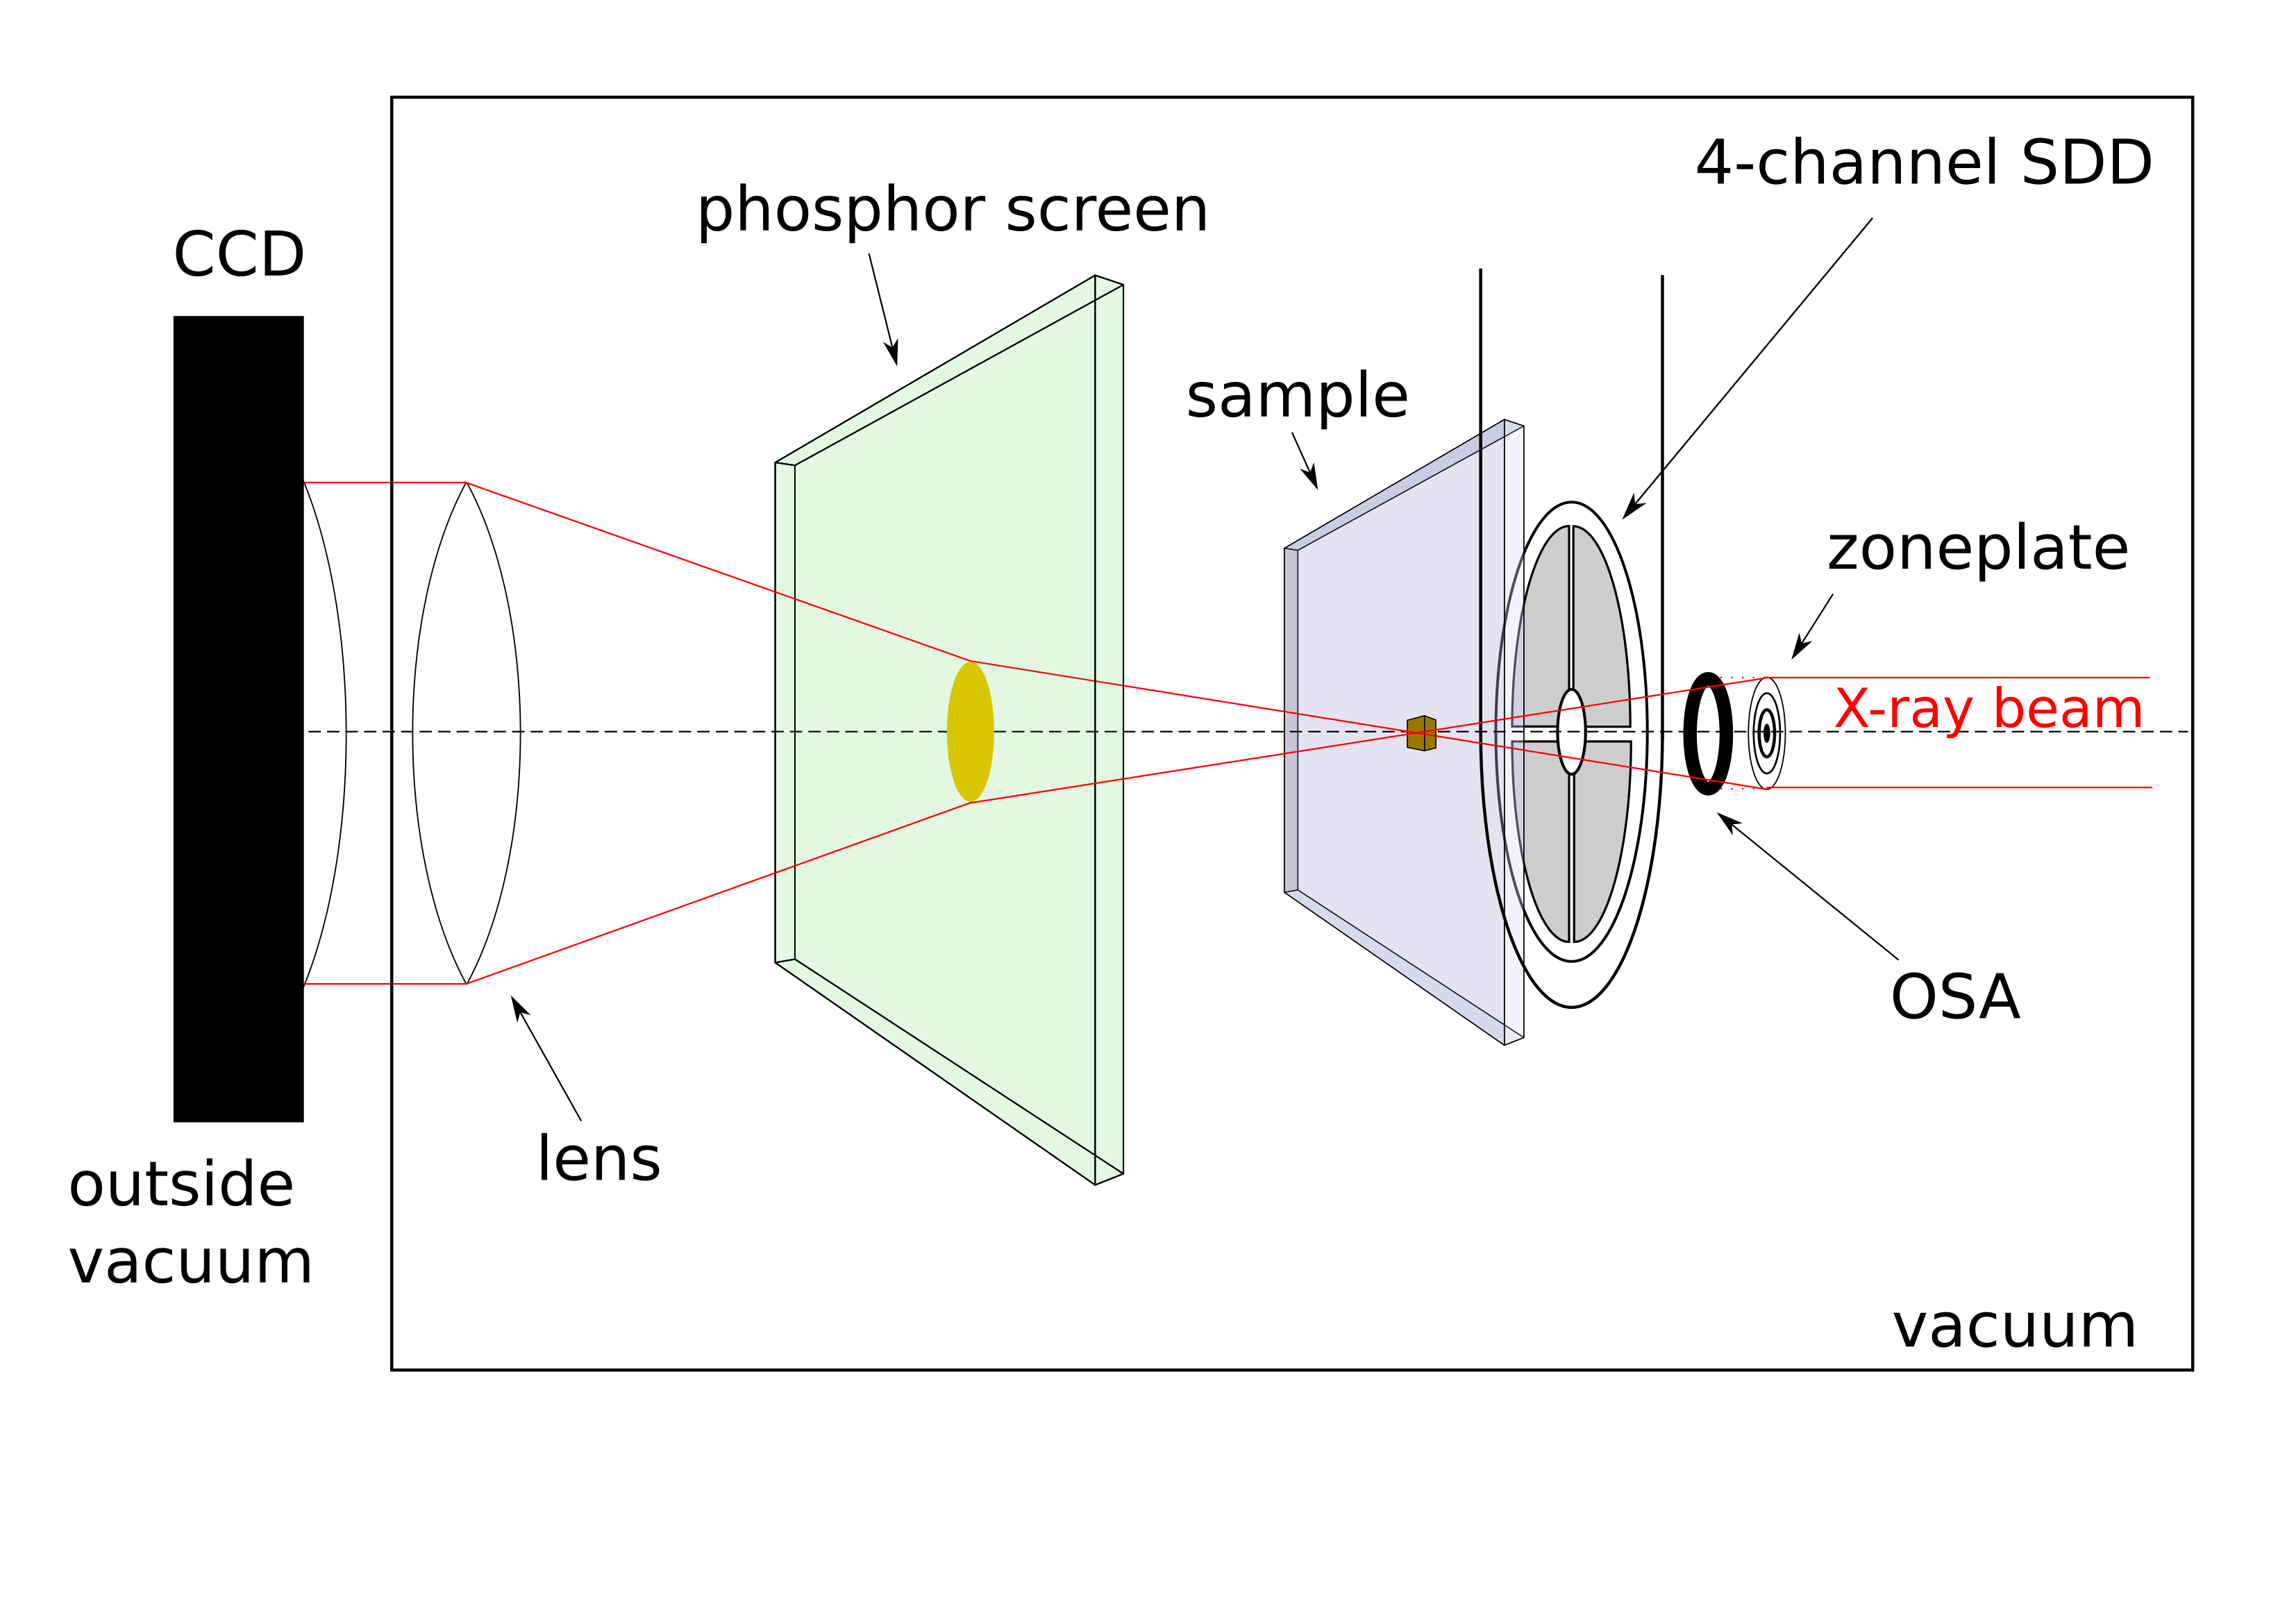
\includegraphics[width=0.9\textwidth]{illustrations/animax-gruppe_hanna.png}
  \caption[Captain Caption]{Captain Caption\cite[S.~40]{hanna}}
  \label{fig:animaxsetup}
\end{figure}




\begin{figure}[H]
\centering
\def\svgwidth{\textwidth}
\input{illustrations/detektorschnitt_hanna.pdf_tex}
  \caption[Captain Caption]{Captain Caption\cite[S.~43]{hanna}}
  \label{fig:quaddetektor}
\end{figure}